% [3~v\textsuperscript{o}]
\pstart% PR: Normal einrücken, bitte.
\textso{Lemme.}
\pend
\pstart
\noindent% PR: Diesen Absatz bitte gar nicht einrücken.
\textso{Les accroissemens du temps en chaque endroit du lieu,
sont en raison reciproque des vistesses}\protect\index{Sachverzeichnis}{vitesse}\textso{,
que le mobile}\protect\index{Sachverzeichnis}{mobile}\textso{
y a.}
\pend
\pstart 
\noindent% PR: Diesen Absatz bitte gar nicht einrücken.
Soit le lieu ou l'espace $\displaystyle EA$ divis\'{e} en parties egales entre elles moindres qu'aucune ligne donn\'{e}e,
$\displaystyle EB.$ $\displaystyle B(B).$ $\displaystyle (B)P$.
Je dis, que les parties du temps
(:~qui seront aussi moindres
\pend
\newpage
\pstart\noindent qu'aucun temps donn\'{e}~:)
dans lesquelles ces parties de l'espace sont parcourues,
seront entre elles, en raison reciproque des vistesses avec lesquelles le mobile parcourt les dites parties de l'espace:
parce que generalement les espaces estant \'{e}gaux,
comme le sont icy les parties,
$\displaystyle EB.$ $\displaystyle B(B).$ $\displaystyle (B)P.$
les temps sont en raison reciproque des vistesses.
Or ces parties du temps, sont ce que j'appelle les accroissemens du temps, en chaque endroit de l'espace.
\pend
\pstart% PR: Normal einrücken, bitte.
Theoreme III.
\pend
\pstart
\noindent% PR: Diesen Absatz bitte gar nicht einrücken.
\textso{Les accroissemens du temps, en chaque endroit du lieu,
qui retarde par tout \'{e}galement un mouuement uniforme en soy m\^{e}me,
pourront estre representez par les appliqu\'{e}es
}[$\displaystyle EG$]\edtext{}{\Bfootnote{$\displaystyle EF$ \textit{\ L \"{a}ndert Hrsg.}}}\textso{,
$\displaystyle BD$, $\displaystyle (B)(D)$ etc. de l'Hyperbole
}[$\displaystyle GD(D)Q$]\edtext{}{\Bfootnote{$\displaystyle FD(D)Q$\textit{\ L \"{a}ndert Hrsg.}}}\textso{
men\'{e}es sur $\displaystyle EA.$ espace,
dans lequel tout le mouuement se doit faire,
et qui est partie de l'Asymptote de l'Hyperbole,
dont le centre $\displaystyle A$ est le m\^{e}me avec le point de repos.}
\pend
\count\Bfootins=1000
\pstart
\noindent% PR: Diesen Absatz bitte gar nicht einrücken.
Car\textso{ par le th. 2. }ces accroissemens representez par les
\edtext{lignes, $\displaystyle BD$, $\displaystyle (B)(D)$}{\lemma{lignes,}\Bfootnote{\textit{(1)}\ $\displaystyle EF$, $\displaystyle BD$, $\displaystyle (B)(D)$ \textit{(2)}\ $\displaystyle BD$, $\displaystyle (B)(D)$ \textit{L}}}
paralleles entre elles, sont en raison reciproque des
\edtext{espaces $\displaystyle AB$, $\displaystyle A(B)$}{\lemma{espaces}\Bfootnote{\textit{(1)}\ $\displaystyle AE$, $\displaystyle AB$, $\displaystyle A(B)$ \textit{(2)}\ $\displaystyle AB$, $\displaystyle A(B)$ \textit{L}}}.
par \edtext{consequent $\displaystyle (B)(D)$}{\lemma{consequent}\Bfootnote{\textit{(1)}\ $\displaystyle EF$ \textit{(2)}\ $\displaystyle (B)(D)$ \textit{L}}}
est \`{a} $\displaystyle BD$
\edtext{comme $\displaystyle AB$ \`{a} [$\displaystyle A(B).$]}{\lemma{comme}\Bfootnote{%
\textit{(1)}\ $\displaystyle A(B)$ \`{a} $\displaystyle AE$ %
\textit{(2)}\ $\displaystyle AB$ \`{a} $\displaystyle AB.$ \textit{L ändert Hrsg.}}}
donc le rectangle $\displaystyle DBA$ est \'{e}gal
\edtext{au rectangle $\displaystyle (B)(D)A.$}{\lemma{au rectangle}\Bfootnote{\textit{(1)}\ $\displaystyle FEA.$ \textit{(2)}\ $\displaystyle (B)(D)A.$ \textit{L}}}
et de m\^{e}me prenant le point $\displaystyle (B)$ quelconque au lieu du point $\displaystyle B.$
le rectangle $\displaystyle (D)(B)A$, est \'{e}gal au dit rectangle
\edtext{fixe $\displaystyle DBA.$}{\lemma{fixe}\Bfootnote{\textit{(1)}\ $\displaystyle FEA.$ \textit{(2)}\ $\displaystyle DBA.$ \textit{L}}}
et par consequent le lieu de tous les
\edtext{points, $\displaystyle D.(D)$}{\lemma{points,}\Bfootnote{\textit{(1)}\ $\displaystyle F.D.(D)$ \textit{(2)}\ $\displaystyle D.(D)$ \textit{L}}}
sera la courbe de l'Hyperbole.
\pend
\pstart% PR: Normal einrücken, bitte.
Theoreme IV.
\pend
\pstart
\sloppy
\noindent% PR: Diesen Absatz bitte gar nicht einrücken.
\textso{Le m\^{e}me estant pos\'{e} les temps m\^{e}mes,
employez \`{a} parcourir une certaine partie de l'espace,
comme $\displaystyle EB$ ou $\displaystyle E(B)$ seront representez par les portions }%
\edtext{\textso{hyperboliques }[$\displaystyle GEBDG.$]%
\textso{ $\displaystyle GE(B)(D)G$}}{\lemma{\textso{hyperboliques}}\Bfootnote{%
\textit{(1)}\ \textso{$\displaystyle FEBDF.$ $\displaystyle FE(B)(D)F$} %
\textit{(2)}\ \textso{$\displaystyle GEBDF.$ $\displaystyle GE(B)(D)G$} \textit{L ändert Hrsg.}}}%
\textso{ comprises entre
}\edtext{\textso{deux appliqu\'{e}es, }}{\lemma{\textso{deux}}\Bfootnote{\textit{(1)}\ \textso{ordonn\'{e}es} \textit{(2)}\ \textso{appliqu\'{e}es,} \textit{L}}}\textso{dont }\edtext{\textso{l'une $\displaystyle EG$ passe}}{\lemma{\textso{l'une}}\Bfootnote{ \textbar\ \textit{(1)}\ \textso{$\displaystyle EF$} \textit{(2)}\ \textso{$\displaystyle EG$} \textit{erg.}\ \textbar\ \textso{passe} \textit{L}}}\textso{
par $\displaystyle E$ point d'o\`{u} le mobile est parti,
l'autre $\displaystyle BD$ ou $\displaystyle (B)(D)$ par $\displaystyle B$ ou $\displaystyle (B)$ o\`{u} le mobile est arriv\'{e}.}
\pend
\count\Bfootins=1200
%\newpage
\pstart 
\noindent% PR: Diesen Absatz bitte gar nicht einrücken.
Car les accroissemens du temps estant representez par les appliqu\'{e}es
[$\displaystyle EG$]\edtext{}{\Bfootnote{$\displaystyle EF$\textit{\ L \"{a}ndert Hrsg.}}},
$\displaystyle BD$, $\displaystyle (B)D$ etc. et une infinit\'{e} d'autres entre elles,
par le\textso{ th. 3. }les sommes des dites accroissements ou les temps employez depuis quelque point,
comme $\displaystyle E$,
seront representez par la somme des dites ordonn\'{e}es
depuis celle qui est prise pour la premiere,
\edtext{comme $\displaystyle EG$}{\lemma{comme}\Bfootnote{\textit{(1)}\ $\displaystyle EF$ \textit{(2)}\ $\displaystyle EG$; \textit{L}}};
c'est \`{a} dire par les espaces compris entre la premiere, et celle qui est \`{a} present la derniere,
c'est \`{a} dire qui passe par le point $\displaystyle B$ ou $\displaystyle (B)$ o\`{u} le mobile est arriv\'{e},
s\c{c}avoir \edtext{entre $\displaystyle EG$}{\lemma{entre}\Bfootnote{\textit{(1)}\ $\displaystyle EF$ \textit{(2)}\ $\displaystyle EG$ \textit{L}}}
et $\displaystyle BD$ ou $\displaystyle (B)(D)$, c'est \`{a} dire par les
\edtext{espaces $\displaystyle GEBDG.$ $\displaystyle GE(B)(D)G$.}{\lemma{espaces}\Bfootnote{\textit{(1)}\ $\displaystyle FEBDF.$ $\displaystyle FE(B)(D)F.$ \textit{(2)}\ $\displaystyle GEBDG.$ $\displaystyle GE(B)(D)G$. \textit{ L}}}
\pend
\pstart% PR: Normal einrücken, bitte.
Theoreme V.
\pend
\pstart
\noindent% PR: Diesen Absatz bitte gar nicht einrücken.
\textso{Si le mouuement d'un corps est uniforme en soy m\^{e}me,
mais retard\'{e} \'{e}galement par le lieu
}\edtext{\textso{o\`{u} il passe, }}{\lemma{\textso{o\`{u}}}\Bfootnote{\textit{(1)}\ \textso{le mobile passe} \textit{(2)}\ \textso{ il passe,} \textit{L}}}\textso{les espaces $\displaystyle BA$ ou $\displaystyle (B)A$ qui restent \`{a} parcourir jusqu'au point de
}\edtext{\textso{repos $\displaystyle A$ depuis le}}{\lemma{\textso{repos $\displaystyle A$}}\Bfootnote{\textit{(1)}\ \textso{jusqu'au} \textit{(2)}\ \textso{depuis le} \textit{L}}}\textso{
point }\edtext{\textso{$\displaystyle B$ ou $\displaystyle (B)$}}{\lemma{}\Bfootnote{\textso{$\displaystyle B$ ou $\displaystyle (B)$} \textit{erg. L}}}\textso{
o\`{u} le mobile est arriv\'{e}, estant comme les nombres;
les temps qui restent
}\edtext{\textso{\`{a} employer}}{\lemma{\textso{\`{a}}}\Bfootnote{\textit{(1)}\ \textso{parcourir} \textit{(2)}\ \textso{employer} \textit{L}}}\textso{
jusqu'\`{a} un certain point, $\displaystyle P$ pris en de\c{c}a du point de repos,
seront comme les Logarithmes des raisons de ces nombres, $\displaystyle BA$ ou $\displaystyle (B)A$,
\`{a} $\displaystyle PA$, distance de ce point $\displaystyle P$ du point de repos, prise pour l'unit\'{e}.}
\pend
\count\Bfootins=1200
\count\Afootins=1200
\pstart
\noindent% PR: Diesen Absatz bitte gar nicht einrücken.
Car on s\c{c}ait que les droites $\displaystyle AP$, $\displaystyle AB$, $\displaystyle A(B)$, $\displaystyle AE$, estant en progression Geometrique continuelle,
les portions Hyperboliques $\displaystyle QP(B)(D)Q$, $\displaystyle (D)(B)BD(D)$,
[$\displaystyle DBEGD$]\edtext{}{\Bfootnote{$\displaystyle DBEFD$\textit{\ L \"{a}ndert Hrsg.}}}
seront \'{e}gales, et par consequent non
\edtext{seulement}{\lemma{}\Afootnote{\textit{Im Text, nach} seulement: NB\vspace{-8mm}}}
\edtext{les portions}{\lemma{les}\Bfootnote{\textit{(1)}\ espaces \textit{(2)}\ portions \textit{L}}}
\edtext{Hyperboliques [$\displaystyle GEBDG$],
$\displaystyle GE(B)(D)G$, [$\displaystyle GEPQG$]}{\lemma{Hyperboliques}\Bfootnote{%
\textit{(1)}\ $\displaystyle FEBDF$, $\displaystyle FE(B)(D)F$, $\displaystyle FEPQF$ %
\textit{(2)}\ $\displaystyle GEBDF$, $\displaystyle GE(B)(D)G$, $\displaystyle FEPQG$ \textit{L ändert Hrsg.}}}
ou (par le \textso{th. 4.}) temps employez d\'{e}ja,
mais aussi les portions Hyperboliques $\displaystyle QP(B)(D)Q.$
\edtext{$\displaystyle QPBDQ.$ $\displaystyle QPEGQ$}{\lemma{$\displaystyle QPBDQ.$}\Bfootnote{\textit{(1)}\ $\displaystyle QPEFQ$ \textit{(2)}\ $\displaystyle QPEGQ$ \textit{L}}}
seront en progression Arithmetique,
d'o\`{u} il s'ensuit comme
\edtext{d'autres}{\lemma{d'autres}\Cfootnote{\textsc{N. Mercator}, \cite{00141}\textit{Logarithmotechnia}, London 1668, prop. XIV-XV, S.~28f.
Leibniz hat in seinem Handexemplar der \textit{Logarithmotechnia} beide Theoreme kommentiert:
Siehe \cite{01189}\textit{LSB} VII,~4 N.~3\textsubscript{1}, S.~50f.}}
ont fait voir, que les dites
\edtext{dernieres}{\lemma{}\Bfootnote{dernieres \textit{erg. L}}}
portions Hyperboliques
\edtext{representent les Logarithmes des raisons des nombres $\displaystyle A(B).$ $\displaystyle AB.$ $\displaystyle AE$ \`{a} l'unit\'{e} $\displaystyle AP$. Or elles representent aussi les temps \`{a} employer depuis les points $\displaystyle E$ ou $\displaystyle B$ ou $\displaystyle (B)$ jusqu' au point $\displaystyle P$ (\textso{par le theor. 4})}{\lemma{representent}\Bfootnote{\textit{(1)}\ aussi les temps \`{a} employer depuis les points $\displaystyle E$ ou $\displaystyle B$ ou $\displaystyle (B)$ jusqu'au point $\displaystyle P$ (par le th. 4)
\textit{(2)}\ les Logarithmes [...] \textso{theor. 4}) \textit{L}}}
donc les dits temps seront aussi comme les Logarithmes susdits.
\pend
\pstart% PR: Normal einrücken, bitte.
Theoreme VI.
\pend
\pstart
\sloppy
\noindent% PR: Diesen Absatz bitte gar nicht einrücken.
\textso{Un point mobile estant port\'{e} par deux mouuemens,
dont les lignes de direction font un angle constant entre elles,
l'un de ces deux mouuemens estant et demeurant uniforme,
l'autre estant uniforme en soy m\^{e}me,
mais retard\'{e} \'{e}galement en chaque endroit du lieu
}\edtext{\textso{o\`{u} passe le mobile;}}{\lemma{\textso{o\`{u}}}\Bfootnote{\textit{(1)}\ \textso{il} \textit{(2)}\ \textso{passe le mobile;} \textit{L}}}\textso{
le dit point d\'{e}crira la ligne Logarithmique.}
\pend
\count\Bfootins=1200
\count\Afootins=1200
\pstart
\noindent% PR: Diesen Absatz bitte gar nicht einrücken.
Conceuuons \edtext{dans\textso{ la 2}\textsuperscript{\textso{de}}\textso{ figure,}}{\lemma{}\Afootnote{\textit{Am Rand:} \textso{2de figure}\textsuperscript{[a]} \vspace{2mm}\\
\footnotesize
\textsuperscript{[a]} \textso{2de figure:} Siehe [\textit{Fig. 3}].\vspace{-8mm}}}
une ligne droite immobile $\displaystyle AE$,
et qu'une regle infexible $\displaystyle BF$,
glisse d'un mouuement uniforme, et sans estre retard\'{e},
le long de cette droite $\displaystyle AE$,
gardant tousjours le m\^{e}me angle $\displaystyle FBE$, ou $\displaystyle (F)(B)E$ etc.
et que cependant un autre mobile glisse ou roule sur la
\edtext{regle $\displaystyle BF$}{\lemma{regle}\Bfootnote{\textit{(1)}\ $\displaystyle BG$ \textit{(2)}\ $\displaystyle BF$ \textit{L}}}
de $\displaystyle B$ \edtext{vers $\displaystyle F.$}{\lemma{vers}\Bfootnote{\textit{(1)}\ $\displaystyle G.$ \textit{(2)}\ $\displaystyle F.$ \textit{L}}}
d'un mouuement, uniforme en soy m\^{e}me,
mais retard\'{e} \'{e}galement en chaque endroit de la regle,
jusqu'au point de repos $\displaystyle F$,
en sorte, que pendant que la regle va de $\displaystyle A$ en $\displaystyle B$;
de $\displaystyle B$ en $\displaystyle (B)$ etc.
le mobile sur la regle aille de $\displaystyle B$ en $\displaystyle D$, de $\displaystyle D$ en $\displaystyle (D)$ etc.
Cela pos\'{e}, si les parties $\displaystyle AB$, $\displaystyle B(B)$, $\displaystyle (B)((B))$ etc. sont \'{e}gales entre elles,
les espaces parcourus $\displaystyle AB$, $\displaystyle A(B)$, $\displaystyle A((B))$ etc.
seront en progression Arithmetique:
or les espaces \edtext{parcourus\protect\index{Sachverzeichnis}{espace parcouru}
par un mouuement uniforme
(:~comme est celuy de la regle $\displaystyle BF$, le long de la ligne $\displaystyle AE$~:)
sont comme les temps employez,
donc les temps employez seront aussi en progression Arithmetique}{\lemma{parcourus}\Bfootnote{\textit{(1)}\ sont comme les temps employez, donc les temps employez seront aussi en progression Arithmetique
\textit{(2)}\ par un [...] Arithmetique; \textit{L}}};
et par consequent\textso{ par le th. 5.
}(:~voyez sa demonstration \`{a} l'endroit marqu\'{e} de
\edtext{NB, o\`{u} il est monstr\'{e}, que les temps employ\'{e}s}{\lemma{NB,}\Bfootnote{\textit{(1)}\ que les temps employez
\textit{(2)}\ o\`{u} il [...] employ\'{e}s \textit{L}}}
ou portions qui les
\edtext{representent $\displaystyle GEBDG.$ $\displaystyle GE(B)(D)G.$ $\displaystyle GEPQG$}{\lemma{representent}\Bfootnote{\textit{(1)}\ $\displaystyle FEBDF.$ $\displaystyle FE(B)(D)F.$ $\displaystyle FEPQF$
\textit{(2)}\ $\displaystyle GEBDG.$ $\displaystyle GE(B)(D)G.$ $\displaystyle GEPQG$ \textit{L}}}
\makebox[1.0\textwidth][s]{\edtext{dans la
\edtext{premiere figure}{\lemma{premiere figure}\Cfootnote{Siehe [\textit{Fig. 2}].}}}{\lemma{}\Bfootnote{dans [...] figure \textit{erg. L}}}
estant en progression Arithmetique[,]
les espaces qui restent, $\displaystyle EA$,}
\pend
\pstart
\begin{center}
 \noindent
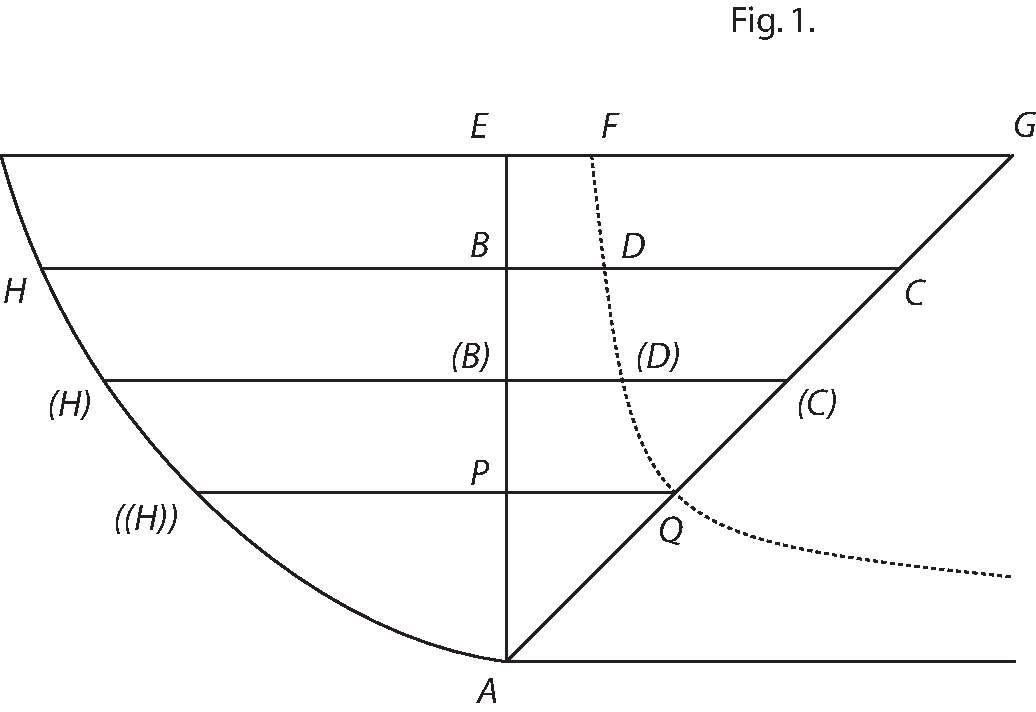
\includegraphics[trim = 0mm -3mm 0mm 10mm, clip, width=0.84\textwidth]{images/lh0350911_004r-d1.pdf}

[\textit{Fig. 1, gestrichen}] 
\end{center}
\pend
\vspace{4mm}
\pstart
\begin{center}
 \noindent
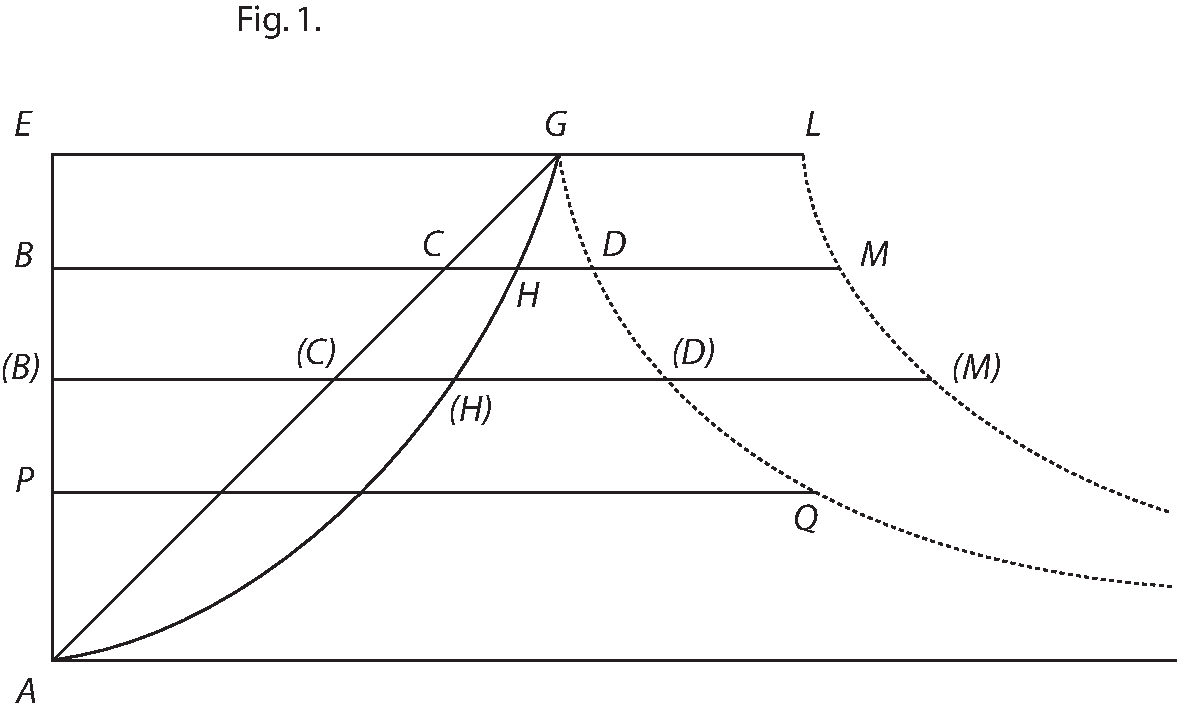
\includegraphics[trim = 0mm 0mm 0mm 10mm, clip, width=0.92\textwidth]{images/lh0350911_004r-d2.pdf}

 \edtext{\hspace{1.8mm}[\textit{Fig. 2}]}{\lemma{[\textit{Fig. 2}]}\killnumber\Bfootnote{\textit{Segment $\displaystyle PQ$ erg. Hrsg.}}}
\end{center}
\pend
\newpage
\pstart
\centering
 \noindent
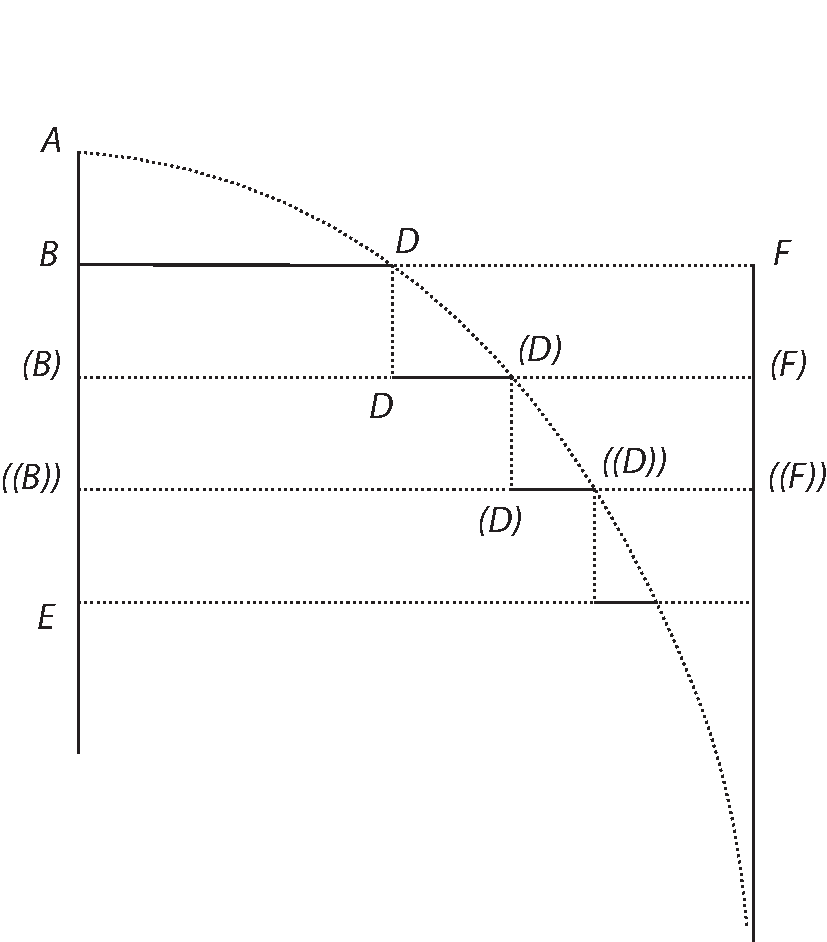
\includegraphics[trim = 0mm 0mm 0mm 0mm, clip, width=0.64\textwidth]{images/lh0350911_004r-d3.pdf}\\
\centering[\textit{Fig. 3}] 
\pend
%\newpage
\vspace{1em} 
\pstart\noindent $\displaystyle (B)A$, \setline{1}$\displaystyle BA$, $\displaystyle PA$
\edtext{dans la \edtext{prem. fig.}{\lemma{prem. fig.}\Cfootnote{Siehe [\textit{Fig. 2}].}}}{\lemma{}\Bfootnote{dans [...] fig. \textit{erg. L}}}
sont en progression Geometrique~:)
et par consequent, dis-je,
les espaces qui restent \`{a} parcourir dans la regle $\displaystyle BF$
(:~de la \edtext{seconde figure}{\lemma{seconde figure}\Cfootnote{Siehe [\textit{Fig. 3}].}}~:)
jusqu'au point de repos $\displaystyle F$,
s\c{c}avoir $\displaystyle DF$, $\displaystyle (D)(F)$, $\displaystyle ((D))((F))$ etc.
ordonn\'{e}es de la droite $\displaystyle F(F)((F))$, sur la courbe $\displaystyle D(D)((D))$
seront en progression Geometrique:
donc le lieu de toutes leurs terminations,
ou de tous les points,
o\`{u} se trouve le mobile,
marchant sur la regle,
et port\'{e} en m\^{e}me temps par la regle,
de la maniere susdite,
sera la ligne Logarithmique.% [4~r\textsuperscript{o}]
% \pend
% \pstart